\section{Reconstruction de CFG}
\label{sec:reconstruction}

  % Limitation des approches de reconstruction de CFG à partir des fichiers
  % sources et nécessité du fichier exécutable pour la reconstruction de CFG.

  Les instructions machine, ou simplement instructions, sont les opérations de
  base codées en langage machine que peut manipuler un processeur. Un fichier
  exécutable contient l'ensemble des instructions d'un programme. Ce type de
  fichier est généralement produit par la compilation des fichiers sources d'un
  programme écrits dans un langage de haut niveau -- un langage de programmation
  -- vers un langage de bas niveau -- le langage machine.

  Certaines méthodes de reconstruction de CFG s'appuient sur les fichiers
  sources des tâches. Cependant, le comportement logiciel qui est effectivement
  constaté à l’exécution n’est pas strictement celui que définissent les
  fichiers sources en langage de haut niveau mais celui que défini le fichier
  exécutable associé en langage de bas niveau. Or, il existe par nature une
  différence d’expressivité entre les langages de haut et de bas-niveau. De
  fait, le processus de compilation équivaut le plus souvent à une fonction de
  traduction non-injective des premiers vers les seconds. De plus, il est très
  fréquent que le processus de compilation inclut une phase d'optimisation du
  fichier exécutable. Les instructions machine y sont modifiées, fusionnées,
  dupliquées, ou réordonnées. L'élément essentiel à une reconstruction précise
  d'un CFG, et a fortiori d'une analyse temporelle précise, est donc le fichier
  exécutable issu de la compilation des fichiers sources du programme considéré.

  \vspace{1em}

  % Définition de CFG et bloc de base

  Un bloc de base est une séquence d'instructions qui n'a qu'un point d'entrée,
  sa première instruction, et qu'un point de sortie, sa dernière instruction.
  Le graphe de flot de contrôle d'un programme est un graphe orienté dans lequel
  les noeuds représentent les blocs de base issus du programme et les
  transitions représentent les enchainements possibles entre les différents
  blocs de base lors de l'exécution du programme. De manière formelle, un CFG
  est un tuple $G = (V, E, u, v)$, où les noeuds $V$ correspondent aux blocs de
  bases, les transitions $E \subset V \times V$ sont les chemins du flot de
  contrôle, $u \in V$ représente le n{\oe}ud d'entrée et $v \in V$ le n{\oe}ud
  de sortie.

  % Principes de recontruction des blocs de base
  
  \begin{figure}[ht]
    \centering
    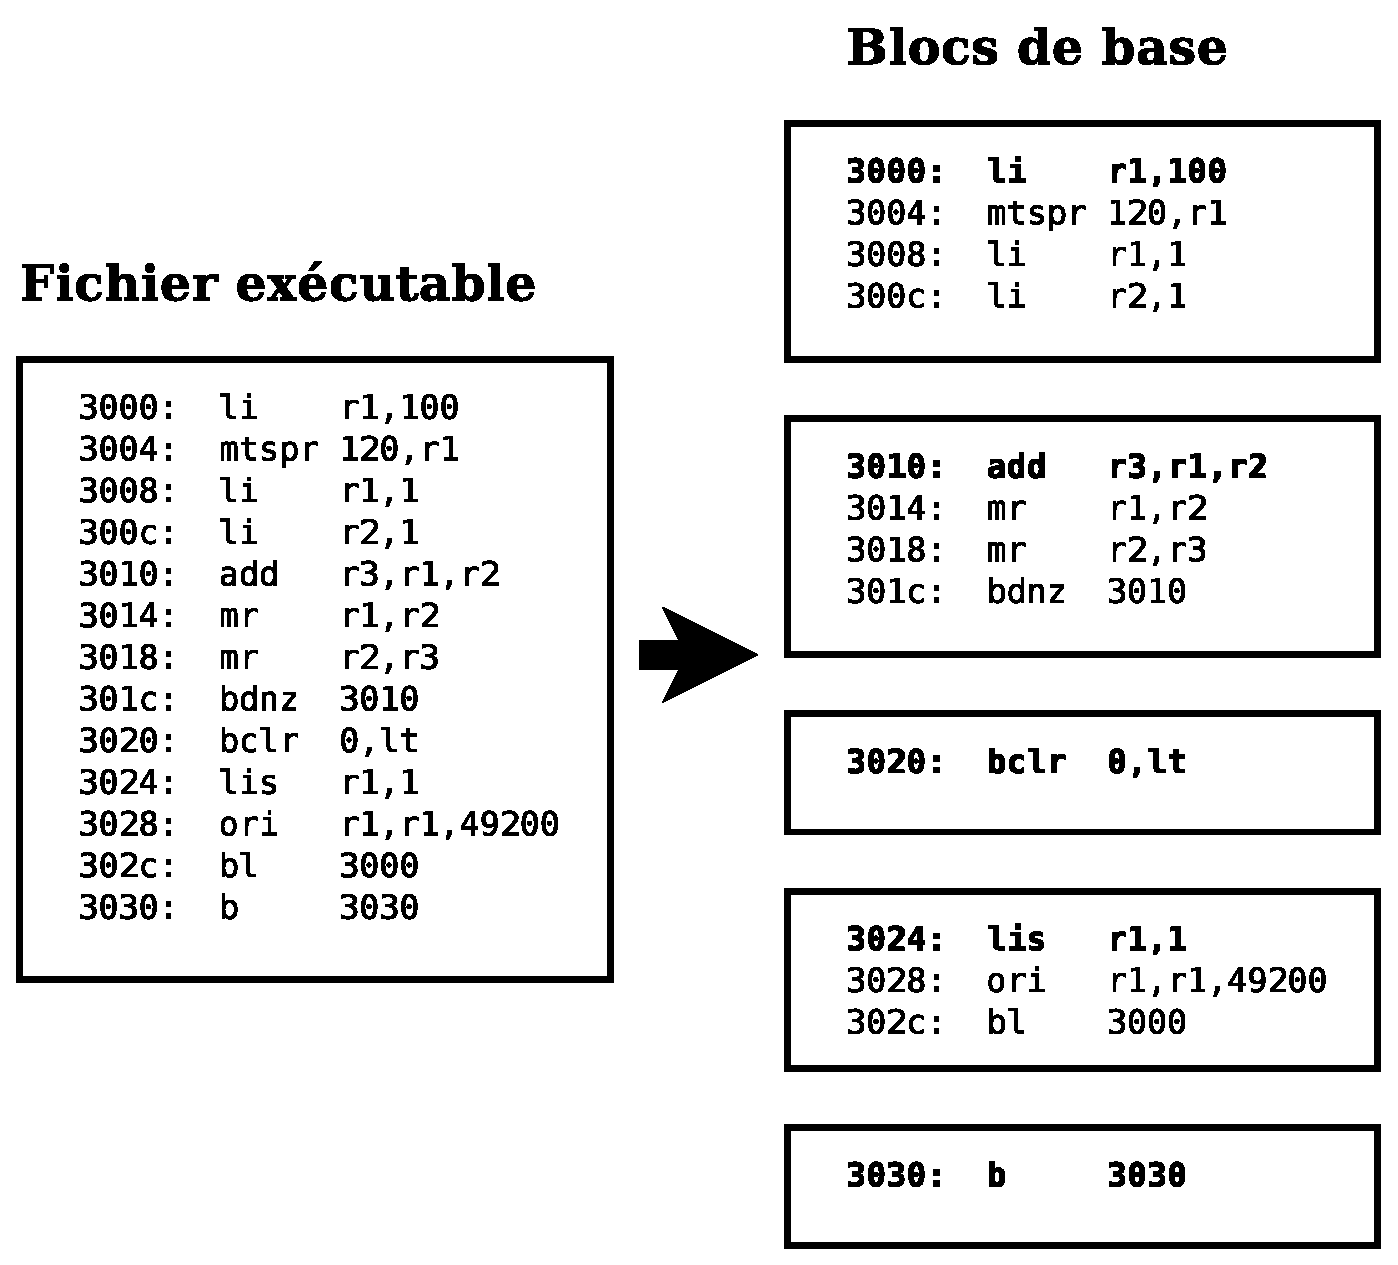
\includegraphics[scale=0.3]{img/recons1.eps}
    \caption{Processus de reconstruction de blocs de base}
    \label{fig:recons1}
  \end{figure}

  Afin de procéder à la reconstruction du CFG d'une tâche, il est tout d'abord
  nécessaire d'en reconstruire les blocs de base. Pour cela il faut identifier
  les points d'entrée de ses différents blocs de base. Une instruction est une
  entrée de bloc de base si elle se trouve être :
    \begin{itemize}
      \item le point d'entrée du programme ;
      \item une cible de saut ;
      \item immédiatement après une instruction de saut ;
      \item la première instruction du fichier exécutable.
    \end{itemize}
  Les blocs de base sont ensuite construits séquentiellement par accumulation
  des instructions se trouvant entre un point d'entrée de bloc de base inclus
  jusqu'au point d'entrée suivant exclus. La figure \ref{fig:recons1} donne un
  exemple d'un telle reconstruction.

  % Utilisation d'un analyseur sémantique de fichiers exécutables pour la
  % reconstruction de CFG.

  Les informations nécessaires à la classification des instructions utiles à la
  reconstruction des blocs de base sont issues d'une analyse syntaxique et
  sémantique du fichier exécutable produite par l'outil \textsc{HARMLESS}
  \cite{KBB12}.
  
  % Principes de recontruction des CFG

  \begin{figure}[ht]
    \centering
    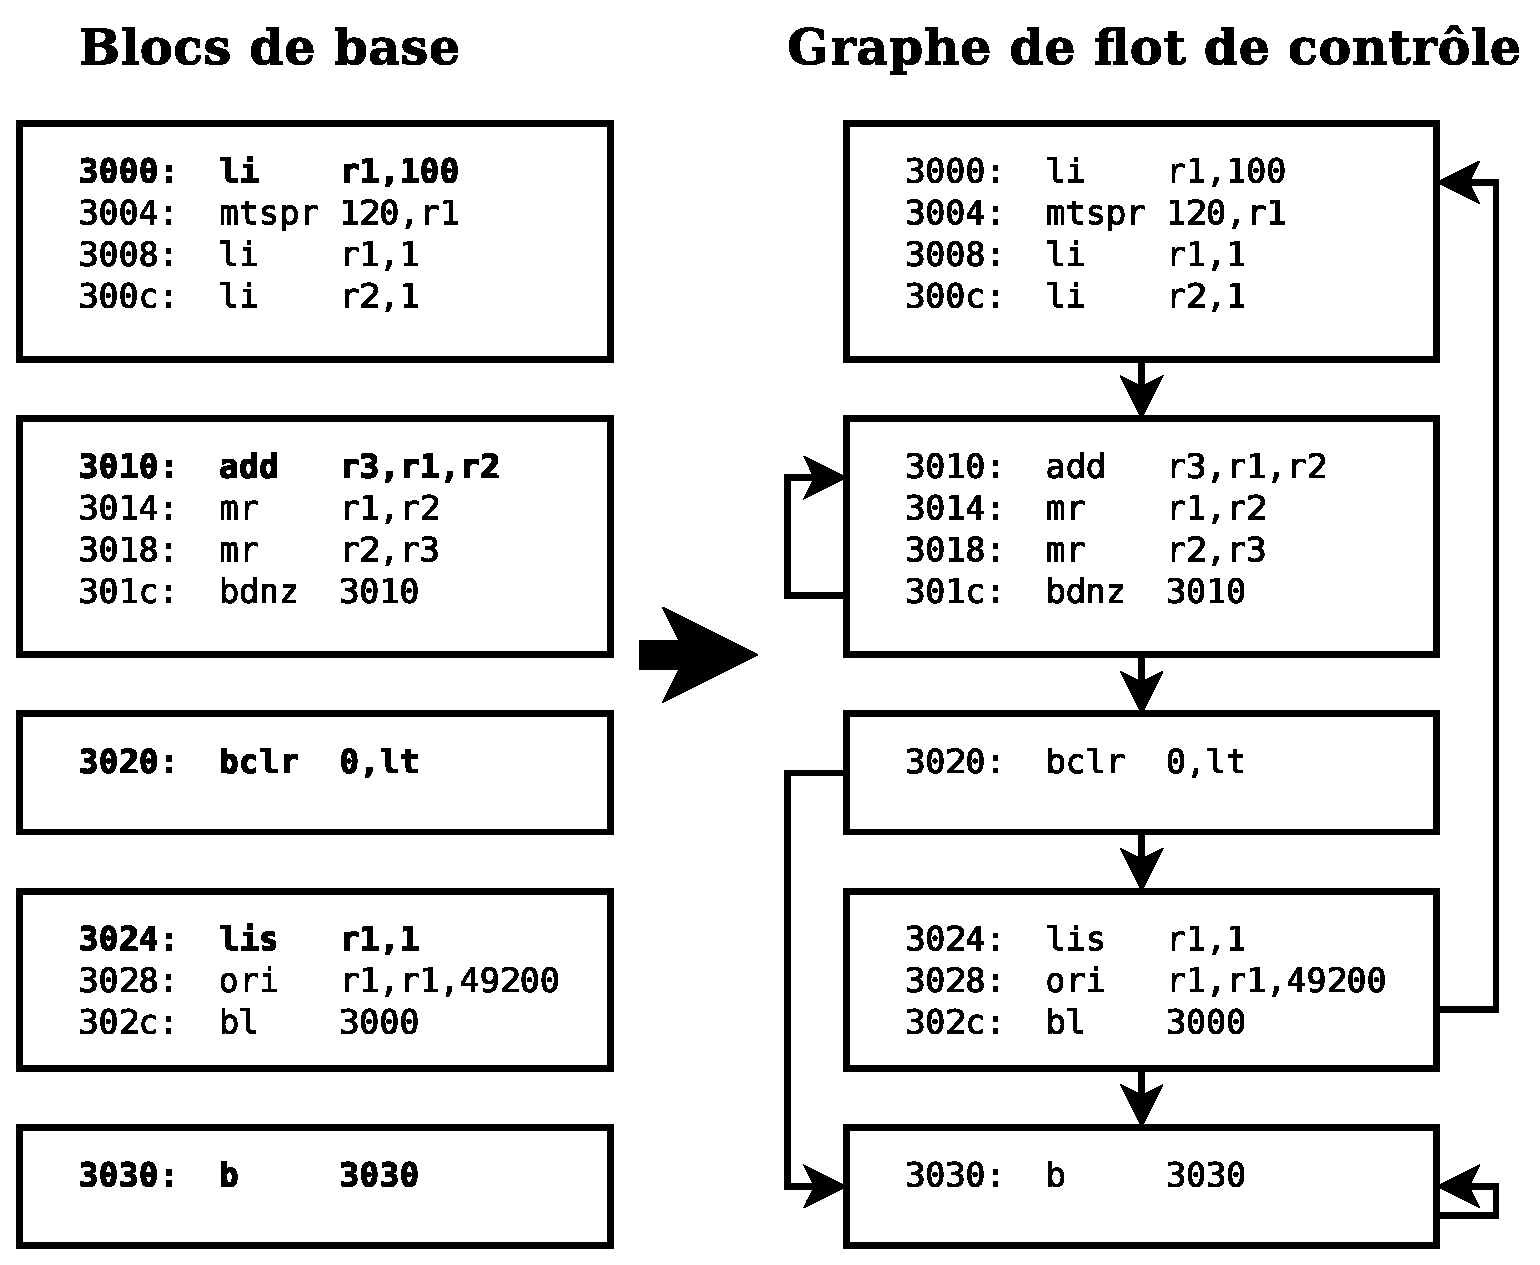
\includegraphics[scale=0.3]{img/recons2.eps}
    \caption{Processus de reconstruction d'un CFG}
    \label{fig:recons2}
  \end{figure}
    
  Pour reconstruire un CFG il est tout d'abord nécessaire d'identifier les
  noeuds. C'est une tâche triviale vis-à-vis de la définition d'un CFG. Il faut
  également identifier le n{\oe}ud d'entrée. C'est le n{\oe}ud correspondant au
  bloc de base issu du point d'entrée du programme. Il faut ensuite en retrouver
  les transitions. Elles sont obtenues itérativement en associant à chaque bloc
  de base les cibles possibles de son point de sortie. La figure
  \ref{fig:recons2} donne un exemple d'un telle reconstruction. Lorsqu'il n'est
  pas trivial de déterminer la cible d'un saut, comme cela peut l'être dans le
  cas de sauts indirects. il est fait usage à ce moment de la reconstruction
  d'un noeud inconnu. Les cibles des ces sauts sont déterminées par la suite.

  %% Utilisation de la propagation de constante pour rafiner le CFG.

  Afin de permettre la déterminaison de certaines cibles de saut il est une
  nouvelle fois fait usage de l'outil \textsc{HARMLESS}. Celui-ci réalise une
  simulation de l'exécution de notre programme sur la plateforme matérielle
  considérée. Il est donc possible de procéder à une propagation de constantes
  permettant de déterminer des plages de valeurs pour certains registres.
